\openingarticle
\def\ppages{\pagerange{Gaggioli:firstpage}{Gaggioli:lastpage}}
\def\shorttitle{Making Better Knives}
\def\maintitle{Making Better Knives: An Experimental Analysis of Projectile Point Technology and Multifunctional Uses}
\def\shortauthor{Amanda Gaggioli}
\def\authormail{amg424@cornell.edu}
\def\affiliation{Cornell University}
\def\thanknote{\footnote{\href{https://cornell.academia.edu/AmandaMary}{Amanda Gaggioli} is an undergraduate student of Classics and Archaeology at Cornell University, USA. She is currently working on a senior thesis, which explores the relationship between humans and their tectonic environment in antiquity, with a specific focus on natural disastrous events occurring in the Bronze Age Aegean. She also works in Cornell’s Laboratory for Aegean and Near Eastern Dendrochronology assisting with the performance of isotopic analyses and the cross-dating of tree-ring samples from Cyprus, Turkey, and Israel that extend and add to the larger Aegean and Near Eastern Dendrochronology Project.}}
%--------------------------------------------------------------
\mychapter{\maintitle}
\begin{center}
	{\Large\scshape\shortauthor \thanknote}\\[1em]
	\email \\
	\affiliation
\end{center}
\vspace{3em}
\midarticle
%--------------------------------------------------------------
\label{Gaggioli:firstpage}

\begin{myabstract}
		\noindent  Testing\marginnote{Astract} the behaviour and function of projectile points broadens the understanding of site function and activities. Projectile point morphology may play a significant role in the efficiency of specific functional uses in Clovis and Cumberland projectile points. This experiment explores the inference that hafted projectile points serve secondary purposes as hafted butchering and cutting tools. The project uses four porcelain casts of Clovis and post-Clovis projectile points, natural animal leg sinew, animal hide glue, and pinewood for hafted handles. The experiment investigates whether a later morphology of projectile points is more effective for use as a knife. The quantitative results reveal the functionality of both Clovis and Cumberland point knives, but determining whether later morphologies served an improved functionality remains in question and requires further experimentation.		

\keywords[Keywords]{Projectile point morphology, experimental archaeology, New World archaeology, use-wear analysis, Pleistocene, Clovis, Cumberland.}
	\end{myabstract}

	%----------------------------------------------------------------------------------------
	%	ARTICLE CONTENTS
	%----------------------------------------------------------------------------------------
	
%	\section{Introduction and Background}
	
\lettrine[nindent=0em,lines=3]{S}{tudies} of the wear and corrosion of projectile points indicate their diagnostic use, whether propelled by hand, spear throwing, or through another formal use. This particular experiment focuses on the wear and tear damage of the hafted area of projectile points to indicate whether later projectile point morphologies would have been functionally more effective as a knife. A need for technological advancement serves as a main factor in the morphology of projectile points over time. This experiment examines two complex research questions. Firstly, did projectile points have secondary uses? Secondly, does projectile point morphology affect the functionality of stone tools? These questions were selected for general interest and also for the range of potential relevant techniques used to address them. With the application of use-wear analyses, the following experiment investigates the inference of prehistoric hafted projectile points serving secondary purposes as hafted butchering and cutting tools through a series of repetitive trials. The project investigates the evolution of projectile point technology and tests the functional efficiency of hafted points used as knives for cutting specific materials. 
	
	
	Stone artefacts are usually by far the most common finds on prehistoric sites. Therefore, stone artefacts provide major sources of information into prehistoric life, since they remain controlled witnesses of prehistoric peoples and their activities \parencite{Cahen_1979}. The history of archaeological investigation into the nature of Pleistocene North America has largely been dominated by the collection and classification of lithic artefacts into the framework of a cultural evolutionary pattern. In order to understand the behaviours of stone tool production, one must use a holistic approach to account for diverse types of variation \parencite{Woods_2011}. Archaeologists use the properties of stone tools to make inferences about the evolution of human behaviour and technology. Experimental and ethnographic research attempts to recapture patterns of prehistoric stone tool production. In addition, experimental research acknowledges the differing environmental and social contexts in which specific tool using behaviour became possible \parencite{Thomas_2011}. Lithic analyses and technical studies tend to focus either upon the identification of prehistoric ethnicity or upon functional patterns that crosscut ethnic boundaries \parencite{Henry_1989}. The contingencies of projectile point manufacture, hafting, use, and rejuvenation create morphological changes. Experiments account for these variables to demonstrate that a single point-type may manifest more than one time-sensitive shape within its primary use. Artefact type reflects conscious preferences and norms on the part of the prehistoric people making and using the artefacts. However, the shape of the projectile does not always disclose the numerous modes of manufacture and use that occurred in the prehistoric context before deposition and recovery from the archaeological record \parencite{Flenniken_1986}. 

	The patterns of damage on stone tools have been shown by both experimental and archaeological studies to be highly diagnostic indicators of various modes of use, and studies that have been conducted to date indicate that this area of research will be an important aspect of behavioural research associated with prehistoric lithic assemblages \parencites{Anderson_2010}{Dockall_1997}. 
Fatigue and abrasive wear patterns associated with the use of point tools indicate diagnostic patterns, some of which are exclusive to the use of projectile armatures, whether propelled by hand, spear thrower, or through the use of a bow. These two types of wear patterns occur on hafted projectile points. Particular worked materials imprint diagnostic types of abrasive and fracture damage on the edges and tips of tools that can be used in the formulation of inferences regarding tool kinematics and task reconstruction. Wear traces are diagnostic of the mechanics of projectile points subjected to both static and dynamic handlings \parencite{Dockall_1997}.
	
	 This experiment utilises similar approaches of technique and method used by past experimental and ethnographic researchers. The design, preparation, and testing were all deeply controlled and standardized in order to deal with projectile point knives and the wear and tear they experience after many repeated uses. The four points used for the experiment were obtained from Dr. David Thulman’s porcelain cast collection. Porcelain material is elementally comparable to chert/flint and other stone materials typically used for the production of prehistoric projectile points. Therefore, the porcelain casts provide a reliable, controlled variable for the testing and analysis of prehistoric projectile points. 
	 
	 The two types of projectiles purposefully chosen were standard Clovis (approximately 11,000\BC) and Cumberland (approximately 9,000\BC) points. The point and tool typologies classify the two distinct hunter-gathering cultures of the Clovis and Cumberland Paleo-Indian people. The Clovis people are often understood to be the first inhabitants of the North America and most likely predecessors of a number of other indigenous cultures, including Cumberland and even living Native American populations \parencite{Haynes_2002}. Both types of Clovis and Cumberland points are found in the New World dispersed throughout North America. Since the Cumberland point dates to a later period than the Clovis point, it is inferred that the design and structure of the Cumberland point would have been better for hafting, and hence would have been functionally more efficient for its second use as a knife \parencite{Anderson_2010}.
	 
	 In particular, the Clovis complex is represented more densely in localities across eastern North America, but there are also distinctive authentications of Clovis technology across western North America \parencite{Morrow_1995}. These points are a relatively large tool that has a short flute (Fig. \ref{fig:gagglioli_Fig1}). The bifacial flute was utilised for hafting purposes. The parabolic shape of the tip curves out into somewhat straight, parallel sides. Overall, the shape of the Clovis point is wide and thick \parencite{Anderson_2010}. Cumberland projectile points are also found throughout North America and date to the Paleo-Indian period. The substantial shape of the point is of a wide V with ears at the distal end of the point and a long, bifacial flute making the point easy to haft. The projectile increases in thickness towards the midpoint with the thickest area at the most proximal point of the fluted area. Overall, the shape of the point is steep and rapidly changes in thickness down the middle and has its greatest width at the midpoint. Cumberland points have a distinct tip that is sharp and long \parencite{Anderson_2010}.

%FIGURE 1 HERE



Through the use-wear analyses, the following experiment investigates the damage on the hafting materials of Clovis and Cumberland projectile point knives with repeated trials of handling and usage. The analyses of variations in wear patterns and damage provides insight into the inference of prehistoric hafted projectile points serving secondary purposes as hafted butchering and cutting tools. 

%\section{Experiment and Methods}
On \marginnote{Experiment and Methods}each of four projectile point knives (two Clovis and two Cumberland), ten trials of one hundred back-and-forth cutting motions along the length of the projectile point were performed on a pinewood block. An Excellence-Precision Balance was used to apply a standard \SI{3.6}{kilogram} of pressure to each knife during each back-and-forth repetition of the experiment. In order to track the changes in the hafting material after each of the ten trials, measurements and photos were taken. Measurements for the change in angle between the point and handle and also the change in length of the knife were recorded in a data table. In total, there were forty attempts with one hundred repetitions for each trial of back-and-forth cutting. 

%\section{Materials}
The \marginnote{Materials} experiment used two of each of the Clovis and Cumberland points, four pinewood handles of the same exact size (Fig. \ref{fig:gagglioli_Fig2}), Whitetail deer hide glue, Whitetail deer leg sinew (Fig. \ref{fig:gagglioli_Fig3}), and an Excellence-Precision Balance to control the amount of pressure applied to the knife during each trial. All points were hafted using the same materials and design. Two of each of the Clovis and Cumberland points were used in order to obtain more data for analysis. Data pertaining to the change in angle between the hafted area of the projectile point and the handle was recorded after each trial of cutting. In addition, the change in length of the knife was recorded to determine whether the pressure from cutting pulled the projectile point from the hafting material.

% BEGIN FIGURES 2 and 3


%\subsection{Knife Handles}
Each\marginnote{Knife Handles} of the four handles was designed and produced to maintain a controlled standard for the experiment. The handles were made using two sections of pinewood measuring \SI{17.78}{\centi\metre} in length and \SI{3}{\centi\metre} in width. The 3cm end sections of the handles were cut and triangulated for hafting purposes. One layer of Scotch® Heavy Duty packing tape held the two sections of wood together leaving a 3cm section at the end of the handle without tape to allow for hafting of the points. The handles were 0.7cm thick taped together.  

%\subsection{Points and Hafting}
The\marginnote{Points and Hafting} porcelain projectile points were made from the casts of original Clovis and Cumberland points. Both Clovis points were \SI{7.7}{\centi\metre} in length and \SI{3.3}{\centi\metre} in width at the widest area of the point with its maximum thickness at \SI{0.7}{\centi\metre}. The Cumberland points both measured \SI{13.7}{\centi\metre} in length and \SI{3}{\cm} at the widest point with its maximum thickness at \SI{0.9}{\centi\metre}. All of the points were hafted in between the two \SI{3}{\cm} triangular wood sections of the handles. The points were held in place using Whitetail deer leg sinew wrapped from the \SI{3}{\centi\metre} line on the handle to the end of the handle. The sinew was then crisscrossed at each corner of the \SI{3}{\centi\metre} length segment and then rewrapped over again from the point of the handle to the \SI{3}{\centi\metre} line on the handle. After wrapping the point and handle with sinew, the \SI{3}{\centi\metre} section of the handle was coated with a layer of Whitetail deer hide glue (Fig. \ref{fig:gagglioli_Fig4}). 
%FIGURE 4 HERE


%\subsection{Wood Block and Scale}
The\marginnote{Wood Block and Scale} testing for the experiment was done on a pinewood block with dimensions of \SI{60}{\centi\metre}$\times$ \SI{15}{\centi\metre}$\times$ \SI{15}{\centi\metre} (base$\times$width$\times$height). The block was placed on an Excellence-Precision Balance in order to maintain a controlled amount of pressure on each knife.

%\section{Measurements}
Measurements\marginnote{Measurements} of the total angles between the handles and projectile points and also the total lengths of the knives were recorded after each trial. In addition, the changes in angle and length for each individual trial were recorded. 
Tracking the changes in angle between the handle and projectile point and modifications in the total length of the knife provided the fundamental data for the overall understanding and evaluation of the results of the experiment. All of the measurements for change in angle between the handle and projectile point were taken using a protractor and recorded in a data table. The angle measurements were taken at the end of the projectile point underneath the hafting materials (Fig. \ref{fig:gagglioli_Fig5}). 
The measurements for change in the length of the knives were also recorded in a data table. Even though all of the handles and each of the Clovis and Cumberland points had the exact same lengths, the lengths of the completed knives varied slightly due to the hafting process. The first Clovis knife was \SI{22.7}{\centi\metre} in length; the second \SI{22.6}{\centi\metre}. The starting length of the Cumberland’s knives were \SI{28.4}{\centi\metre} and \SI{28.7}{\centi\metre} respectively.


%\section{Data and Results}
The\marginnote{Data and Results} following sections dedicated to each type of knife are organized to present the qualitative and quantitative results in a more meaningful and understandable manner. The final comparisons and conclusions follow in a discussion after the individual presentation of each knife type. 

%\subsection{Clovis Point Knife 1 and 2}
Before\marginnote{Clovis Point Knife 1 and 2} testing, the Clovis knives were expected to experience drastic changes in their structure and consequently, their ability to function would diminish as the trials went on. The point’s width, linear shaped confirmed the former expectation that the hafting material would wear and tear at a much quicker rate than the Cumberland knives. However, during the first trials, there were either no changes or only slight changes in the lengths of the knives and angles of the projectiles and handles of the knives. The hide glue and sinew experienced some wear and tear, but the knife remained highly functional. The slight wearing and tearing of the hafting material did not affect the overall sturdiness of the knives. In addition, the functionality of the knives remained the same throughout each of the trials. The measurements for both of the Clovis knives are shown in table \ref{fig:Table1}.

%INSERT TABLE 1 or Fig 6 HERE



%\subsection{Cumberland Point Knife 1 and 2}
Originally,\marginnote{Cumberland Point Knife 1 and 2} the Cumberland point knives were hypothesized to not experience drastic wear and tear on the hafting materials, since the shape at the distal end of the points allowed for easier hafting. A visual analysis of the knives showed only minor wearing or tearing on the glue or sinew of the knives. The measurements demonstrated slight changes in the angles between the handles and projectile points and also in the total lengths of the knives. Overall, the knives remained functional in cutting. The measurements for both of the Cumberland knives are in table \ref{fig:Table2}. 

%INSERT TABLE 2 or Fig 7 HERE

%\section{Results}

%\subsection{Use-Wear Damage of Hafting Material}

In\marginnote{Results\\Use-Wear Damage of Hafting Material} terms of the wear and tear of the hafting materials (Fig. \ref{fig:gagglioli_Fig6}), the Clovis point knives experienced more deterioration and corrosion on the sinew and glue of the hafting portion of the knife. Damage likely occurred due to the wide and linear shape of the Clovis projectile point. During each trial and repetition, the straighter edge of the Clovis point knives rubbed frequently and consistently and in 	
	effect, this created more deterioration after each trial. The wings of the Cumberland point created a narrow gap in the hafted segment of the knife. The narrow gap provided some relief from the stress and friction of the back-and-forth movement during each repetition. Consequently, the hafted portion of the Cumberland point knives did not experience as much scraping for the same action.
	
	%ADD FIGURE 6 or FIG 8 HERE
	
%\subsection{Functionality of Projectile Point Knives}
Despite\marginnote{Functionality of Projectile Point Knives} the differences in the wear and tear of hafting materials between the Clovis and Cumberland point knives, the two types did not vary significantly in their changes of length and angle (Figures \ref{fig:Chart1}; \ref{fig:Chart2} or Charts 1 \& 2). Overall, the modifications were minimal for both knives. During the first few trials the Clovis point knives, no change or very slight change in the angles and lengths of the knives was perceived. The change in angle between the projectile point and the handle was greatest in the second Clovis point knife. However, comparing these differences was not possible to reach significant conclusions based on the ability to function more efficiently as a knife.
	
In terms of reduction in lengths, the first Cumberland point knife experienced the most significant change in the overall length of the knife, which was unexpected based on the hypothesis presented earlier in this paper. Nevertheless, the changes in length likely resulted from the greater length of the Cumberland projectile point in comparison to the Clovis projectile point. The repetitions were done along the length of the entire projectile point. Therefore, the Cumberland point knives experienced a longer repetition than the Clovis point knives, which may have pulled the Cumberland projectile point from the haft at a slightly quicker rate than the Clovis points. 

The constant, high pressure and repetitive trials applied to the knives created only minor variations in the structure of the knives. In comparison, the changes in angles and lengths of all the knives were not significant enough to determine whether later morphologies of projectile points were technologically better for secondary uses of projectile points. All the remained knives highly functional throughout the entire experiment. 

	%ADD CHART 1 or FIG 9 HERE
	


%\section{Discussion}
Overall,\marginnote{Discussion} each of the four knives remained highly functional after many repetitions and trials. Based on comparisons of the measurements in angle and length, determining whether the later morphology in design and structure of the Cumberland point would have been functionally more efficient for its secondary use as a knife remains inconclusive. Further research and testing is needed to determine whether later morphologies of projectile points functioned more efficiently as hand tools.

This experiment included many variables, and in the future, the controlled variables of this experiment could be altered to conduct similar types of research. For example, testing prehistoric hand tools on different types of materials, rather than only a controlled wood block, has potential to provide insight into the distinct uses of knives and other hand tools in prehistoric times. 

Future research can find the results of this analysis useful in other types of experimentation that aim to test the morphology and multifunctional uses of projectile points. This experiment and research can represent a stepping-stone into the exploration of the secondary uses of projectile points. Overall, the results provide strong evidence in support for the inference that hafted projectile points indeed served secondary purposes as hafted butchering and cutting tools. 


In spite of the efforts to keep the experiment controlled, a few uncertain variables need to be accounted for. Even though a scale was used to maintain a consistent \SI{3.6}{\kilogram} of pressure on the knives during each trial, there were a number of minor fluctuations while performing the repetitions of the back-and-forth movements on the knives. In addition, the angle at which the knife was cutting varied slightly throughout the experiment. 
		An effort to keep the knives at the same cutting angle was attempted; however measures were not taken to keep this exact. Additionally, the space in between the 
	two wood segments on the hafting end of the knife varied slightly due to the taping of the handles in preparation for the experiment (Fig. \ref{fig:gagglioli_Fig7}). Lastly, since use-wear patterns on the blades themselves were not visible upon objective observation alone, one may propose a necessity to utilize microscopic analyses in order to examine the use-wear on the blades of the knives. This could then be used in conjunction with analyses of the use-wear in the hafting material. Overall, these uncertain factors are minimal but their recognition is necessary, especially for future research and experimentation.
	
		%ADD Figure 7 FIG 10 HERE
	
%\section{Conclusion}
Overall,\marginnote{Conclusion} the analyses of damage patterns on Clovis and Cumberland points provide valuable insight into the functionality of projectile point knives. Although, determining whether later morphologies served an improved functionality remains in question, the results, nevertheless, reveal a strong likelihood that Paleo-Indian cultures employed projectile points as secondary hand tools. The efficient strength and durability of the knives throughout many repeated trials adds to a more broad comprehension of human behaviours with stone tools. Incorporating this information about human behaviour with the reconstruction of subsistence strategies in archaeological sites with Clovis or Cumberland points further develops the understanding of a site’s function and activities. 

\myseparator

%\section{Acknowledgements}
The\marginnote{Acknowledgements} author owes a great thanks to Dr. David Thulman for help with experimental construction and setup and also for providing vital materials for the project. Without his supervision and expertise the experiment would not have been successful. Finally, thanks to all the readers.


\begin{figure}[!p]
	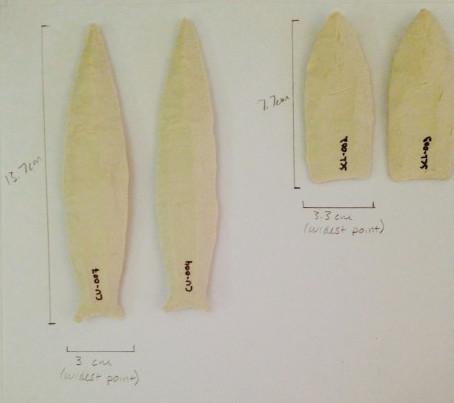
\includegraphics[width=\linewidth]{figures/gagglioli_Fig1}
	\centering
	\caption{Cumberland (left) and Clovis (right) points.}
	\label{fig:gagglioli_Fig1}
\end{figure}	

\begin{figure}[!p]
	\centering
	\begin{minipage}{0.45\textwidth}
		\centering
		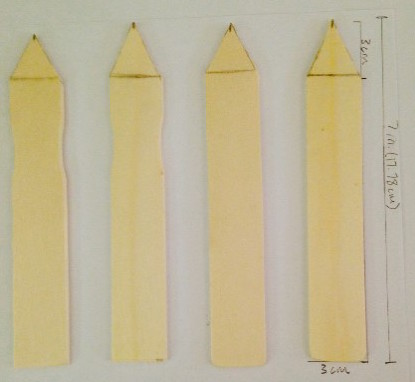
\includegraphics[width=1.15\linewidth]{figures/gagglioli_Fig2}
		\caption{Four Pinewood handles crafted for experimental purposes.}
		\label{fig:gagglioli_Fig2}
	\end{minipage}\hfill\noindent 
	\begin{minipage}{0.4\textwidth}
		\centering
		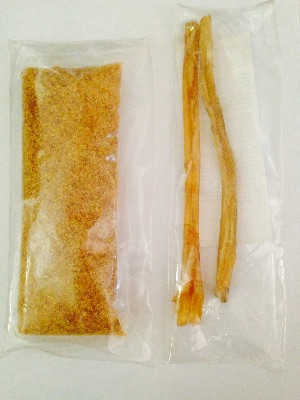
\includegraphics[width=\linewidth]{figures/gagglioli_Fig3}
		\caption{Animal hide glue (left) and sinew (right).}
		\label{fig:gagglioli_Fig3}
	\end{minipage}
\end{figure}

\begin{figure}[!p]
	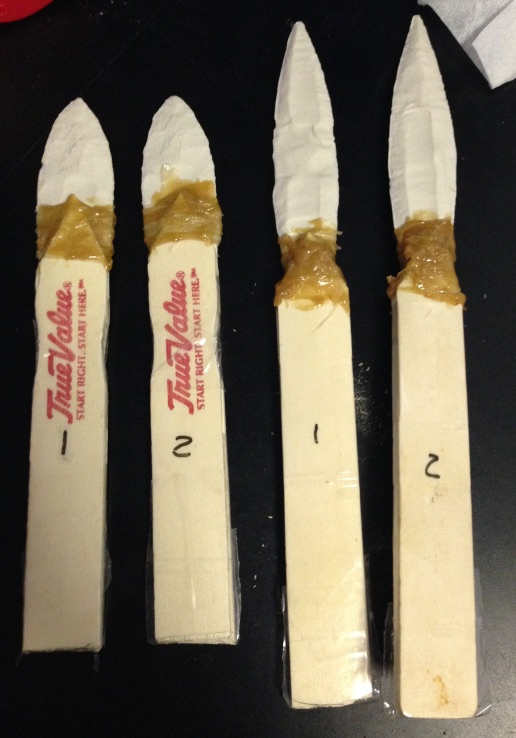
\includegraphics[width=\linewidth]{figures/gagglioli_Fig4}
	\centering
	\caption{Clovis (left) and Cumberland (right) point knives.}
	\label{fig:gagglioli_Fig4}
\end{figure}

\begin{figure}[!p]
	\centering
	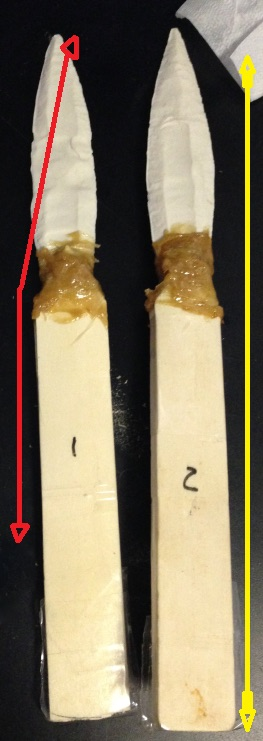
\includegraphics[width=.5\linewidth]{figures/gagglioli_Fig5}
	\caption{The red arrows demonstrate where angles were measured and the yellow arrows demonstrate where the length was measured.}
	\label{fig:gagglioli_Fig5}
\end{figure}

\begin{figure}[!p]
	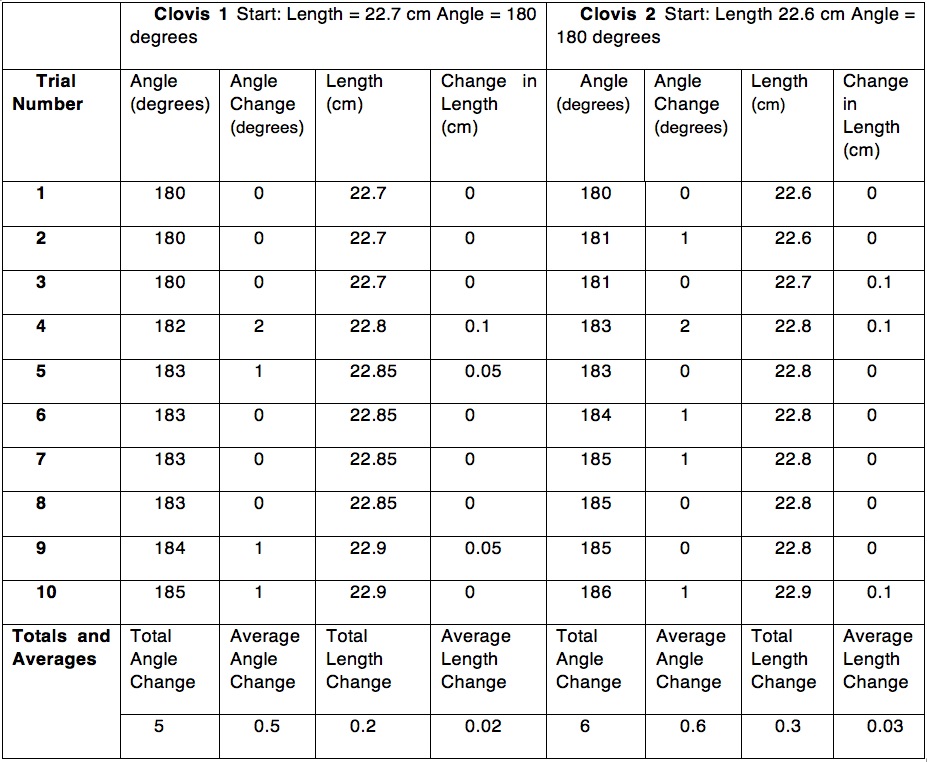
\includegraphics[width=\linewidth]{figures/gagglioli_Table1.png}
	\centering
	\captionof{table}{Trial Data for Clovis Points.}
	\label{fig:Table1}
%\end{figure}
%
%\begin{figure}[!p]
	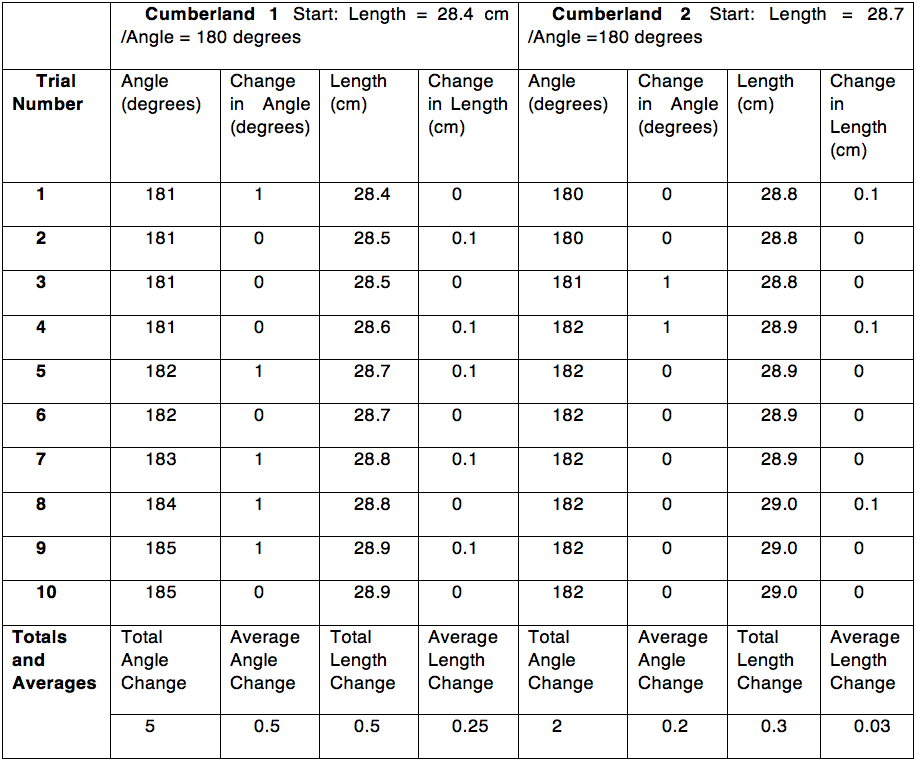
\includegraphics[width=\linewidth]{figures/gagglioli_Table2.png}
	\centering
	\captionof{table}{Trial Data for Cumberland Points.}
	\label{fig:Table2}
\end{figure}

\begin{figure}[!p]
	\centering
	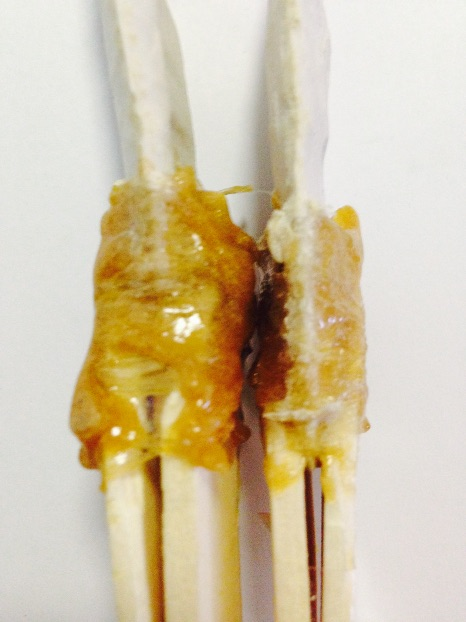
\includegraphics[width=.95\linewidth]{figures/gagglioli_Fig6}
	\caption{Hafting material: Cumberland (left) and Clovis (right).}
	\label{fig:gagglioli_Fig6}
\end{figure}

\begin{figure}[!p]
	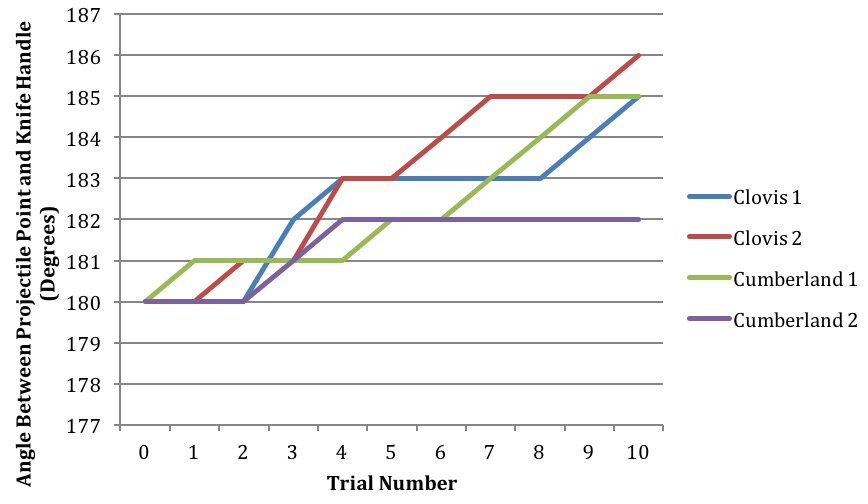
\includegraphics[width=\linewidth]{figures/gagglioli_Chart1}
	\centering
	\caption{(Chart 1) The Change in Angle Between the Projectile Point and Knife Handle.}
	\label{fig:Chart1}
\end{figure}


%ADD CHART 2 FIG 10 HERE

\begin{figure}[!p]
	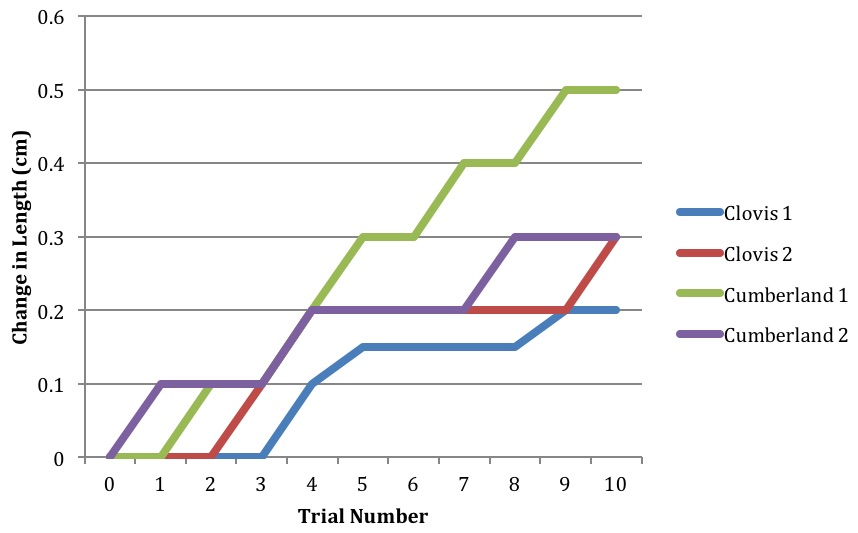
\includegraphics[width=\linewidth]{figures/gagglioli_Chart2}
	\centering
	\caption{(Chart 2) Change in Length of Each Knife.}
	\label{fig:Chart2}
\end{figure}

\begin{figure}[!p]
	\centering
	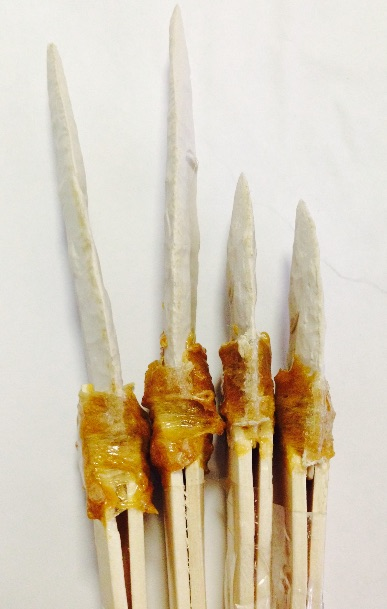
\includegraphics[width=\linewidth]{figures/gagglioli_Fig7}
	\caption{Spacing in between two wood segments. Cumberland (left) and Clovis (right).}
	\label{fig:gagglioli_Fig7}
\end{figure}
\clearpage
	%----------------------------------------------------------------------------------------
	%	REFERENCE LIST
	%----------------------------------------------------------------------------------------
\printbibliography[heading=subbibnumbered] 
\label{Gaggioli:lastpage}
%----------------------------------------------------------------------------------------
\closingarticle